%第4章:実験結果・考察
本章ではV字モデル開発に従って実装を行った。ここでは具体的な実装方法について述べる。
\section{実装}
 実装に至っては2人のグループで行いエッジ処理側は真鍋樹が行った。ここではサーバ側の実装について述べる。ここではエッジ処理側のことをクライアントと呼ぶ。実装に使用したプログラム言語はクライアント、サーバどちらもPython3を使用した。

\subsection*{サーバ通信}
 クライアントとのデータのやり取りを含めた連携には通信処理が必要不可欠になる。クライアントはセンサが反応したらカメラを起動し複数の画像を撮影する。つまりサーバに送られる画像データは1回につき1枚ではない。つまりクライアントが画像データを送信するデータサイズが不明のため、サーバ側では送信されたデータのどこからどの部分が1つの商品画像データになるのか判断できない。そこで、クライアントは画像データを送信する前に画像データの合計サイズを送信する。サーバは合計サイズ分だけデータを受信すれば続けて2回目のデータ送信が来ても1回目のデータと区別することができる。
クライアントから送られてきた画像データはバイナリ形式になっているのでOpenCVのフォーマットに変換しなおしている。

\subsection*{Yoloによるバーコード領域特定}
 Yoloを使用した理由は後述するpyzbar\cite{pyzbar}.の識別精度にある問題があったためである。pyzbar\cite{pyzbar}.は近距離で撮影したバーコードの画像の認識はうまくいくが、距離が離れると識別しなくなる。これは画像の中に占めるバーコード部分が少なくなってしまい認識がうまくいかないためと思われる。そこでYoloを使用し、画像からバーコードの部分のみの座標を取得する。バーコードの部分のみをpyzbarに渡すことで距離が離れていても近距離で撮影したのと同じ効果が得られるようになった。学習にはバーコードの画像を約2000枚用意した。
 
 Yoloの実行はサーバ側で行う。当初クライアント側であるRaspberryPiでYoloを実行すればサーバは不要になり通信におけるタイムラグもなくなることが期待されたが、残念ながらラズパイの性能ではYoloを高い識別精度を保ったままリアルタイムに動作させることは性能上難しかったためサーバで行うことになった。

\subsection*{DBを使用した商品情報の管理}
 カゴの中の商品を管理と、商品自体の情報の管理にDBを使用した。MariaDBを使用した。カゴDBの構造を表に示す。

%%%%カゴDB表とそれぞれの意味

次に商品DBの機能を表に示す。
%%%商品DB


\subsection*{決済システム}
 設計では決済システムが動作するのはユーザが退店する際に自動で行われることになっているがその機能を実装するには時間の都合上難しいと判断したため、仮の決済用Webページを作成して代用している。ページ作成にはPHPを使用している。

\section{検証}
 V字モデルに従って4.1節で述べた実装部分に関するテストを行うことで要件を満たしているかどうかを確認する。以下にそれぞれのテスト項目を表で示す。

\subsection*{サーバ通信}
 サーバ通信の検証で行った単体テストを以下の表\ref{server_test}に示す。
\begin{figure}[htbp]
\centering
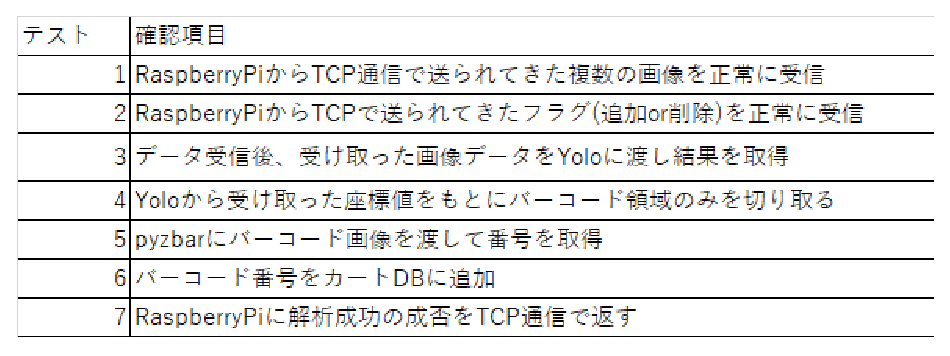
\includegraphics[width=12cm]{./pic/server_test.eps}
\caption{サーバ通信単体テスト}
\label{server_test}
\end{figure}

\subsection*{Yoloによるバーコード領域特定}
 Yoloにおけるバーコード検知の検証で行った単体テスト項目を以下の表\ref{yolo_test}に示す。
\begin{figure}[htbp]
\centering
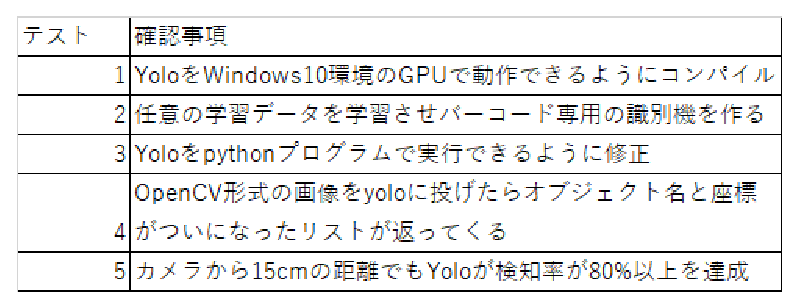
\includegraphics[width=12cm]{./pic/yolo_test.eps}
\caption{Yoloによるバーコード領域特定単体テスト}
\label{yolo_test}
\end{figure}

\subsection*{DBを使用した商品情報の管理}
 DBを使用した商品情報の管理の単体テストは

\subsection*{決済システム}
 決済システムにおける単体テストを以下の\ref{db_test}に示す
\begin{figure}[htbp]
\centering
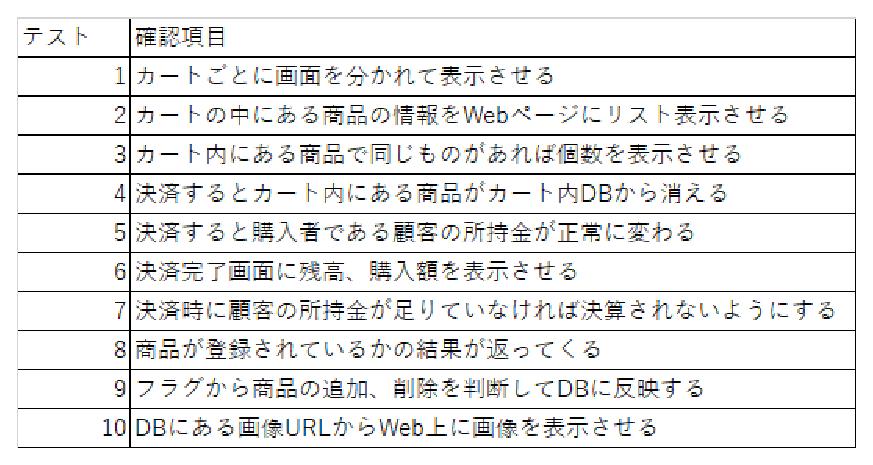
\includegraphics[width=12cm]{./pic/db_test.eps}
\caption{決済システム単体テスト}
\label{db_test}
\end{figure}


